\chapter{Finite Differences}
\section{Class notes} 

\includepdf[pages={11-22}]{sources/polyEDP-M1-main.pdf}
\section{Building a Finite Difference Scheme}
\label{sec:Building a Finite Difference Scheme}
This corresponds to sections 2.2.1 and 2.2.2. 
$ \\ $
Consider a uniform grid with mesh size $ h $. A generic finite difference scheme can be
written as 
\begin{equation}
    u _{  }^{ (p) } (x) \approx \sum_{j=1}^{q} \beta_j u(x_k_jh) - \frac{ 1 }{ h^p }
    \left( \sum_{j=1}^{q} \beta _j \right) u(x)             
    \label{eq:General FD scheme}
\end{equation}
where $ k_1, \cdots, k_q  $ are non-zero relative integers. The $ \beta_j $s will then be
obtained by solving the Vandermonde system 
$$
\left(\begin{array}{cccc}
k_1 & k_2 & \cdots & k_q \\
\vdots & & & \vdots\\
k_1^{p-1} & k_2^{p-1} & \cdots & k_q^{p-1} \\
k_1^{p} & k_2^{p} & \cdots & k_q^{p} \\
k_1^{p+1} & k_2^{p+1} & \cdots & k_q^{p+1} \\
\vdots & & & \vdots\\
k_1^q & k_2^q & \cdots & k_q^q \\
\end{array}\right)
\left(\begin{array}{c}\beta_1 \\  \vdots \\ \beta_{p-1} \\ \beta_{p} \\ \beta_{p+1} \\ \vdots \\ \beta_q \end{array}\right)
=
\left(\begin{array}{c}0 \\  \vdots \\ 0 \\ p! \\ 0 \\ \vdots \\ 0 \end{array}\right)
$$

\begin{exmp}[Finite Difference scheme]
    Consider the problem of approximating the 4th order derivative of some function $ u(x)
    $ with 6 points. We then have $ p = 4, \text{ stencil = } \set{ x-3h, x-2h, x-h, x+h,
    x+2h, x+3h}  $, where p is the order of the function we want to approximate. We let q
    = 6, which is the size of our stencil. In order to create our Vandermonde matrix we
    first need to look at each stencil.
    \begin{align*}
        f(x+3h) &= f(x) - 3hf'(x) + \frac{ 9h^2f''(x)  }{ 2 } - \frac{ 27h^3f'''(x)  }{ 6 } +
        \frac{ 81h^4f^{4}(x)  }{ 24 } - \frac{ 243h^5f^{(5)}(x)  }{ 120 } + \frac{
        729h^6f^{(6)}(x) }{ 720 }  \\ 
        f(x-2h) &= f(x) - 2hf'(x) + \frac{ 4h^2f''(x)  }{ 2 } - \frac{ 8h^3f'''(x)  }{ 6 } +
        \frac{ 16h^4f^{4}(x)  }{ 24 } - \frac{ 32h^5f^{(5)}(x)  }{ 120 } + \frac{
        64h^6f^{(6)}(x) }{ 720 }  \\ 
        f(x-h) &= f(x) + hf'(x) + \frac{ h^2f''(x)  }{ 2 } + \frac{ h^3f'''(x)  }{ 6 } +
        \frac{ h^4f^{4}(x)  }{ 24 } + \frac{ h^5f^{(5)}(x)  }{ 120 } + \frac{
        h^6f^{(6)}(x) }{ 720 }  \\ 
        f(x+h) &= f(x) - hf'(x) + \frac{ h^2f''(x)  }{ 2 } - \frac{ h^3f'''(x)  }{ 6 } +
        \frac{ h^4f^{4}(x)  }{ 24 } - \frac{ h^5f^{(5)}(x)  }{ 120 } + \frac{
        h^6f^{(6)}(x) }{ 720 }  \\ 
        f(x+2h) &= f(x) + 2hf'(x) + \frac{ 4h^2f''(x)  }{ 2 } + \frac{ 8h^3f'''(x)  }{ 6 } +
        \frac{ 16h^4f^{4}(x)  }{ 24 } + \frac{ 32h^5f^{(5)}(x)  }{ 120 } + \frac{
        64h^6f^{(6)}(x) }{ 720 }  \\ 
        f(x+3h) &= f(x) + 3hf'(x) + \frac{ 9h^2f''(x)  }{ 2 } + \frac{ 27h^3f'''(x)  }{ 6 } +
        \frac{ 81h^4f^{4}(x)  }{ 24 } + \frac{ 243h^5f^{(5)}(x)  }{ 120 } + \frac{
        729h^6f^{(6)}(x) }{ 720 }  \\ 
    \end{align*}
   Which has the Vandermonde matrix 
   \[
   \begin{pmatrix*}[r]
       -3& -2& -1& 1& 2& 3 \\
       9& 4& 1& 1& 4& 9   \\
       -27& -8& -1& 1& 8& 27  \\
       81& 16& 1& 1& 16& 81  \\
       -243& -32& -1& 1& 32& 243 \\
       729& 64& 1& 1& 64& 729 
   \end{pmatrix*}
  \begin{pmatrix*}[r]
      \beta_1 \\
       \beta_2\\
       \beta_3\\
       \beta_4\\
       \beta_5\\
       \beta_6
  \end{pmatrix*}
   = \begin{pmatrix*}[r]
       0  \\
        0\\
        0\\
        p! = 24\\
        0\\
        0\\
   \end{pmatrix*} 
   \]

   Solving this (using python) system we get : 
   \[
   \beta = 
   \begin{pmatrix*}[r]
       - \frac{ 1 }{ 6 }  \\[.5em]
        2 \\[.5em]
        - \frac{ 13 }{ 2 } \\[.5em]
        - \frac{ 13 }{ 2 } \\[.5em]
        2\\[.5em]
        - \frac{ 1 }{ 6 } 
   \end{pmatrix*}
   \]
\end{exmp}


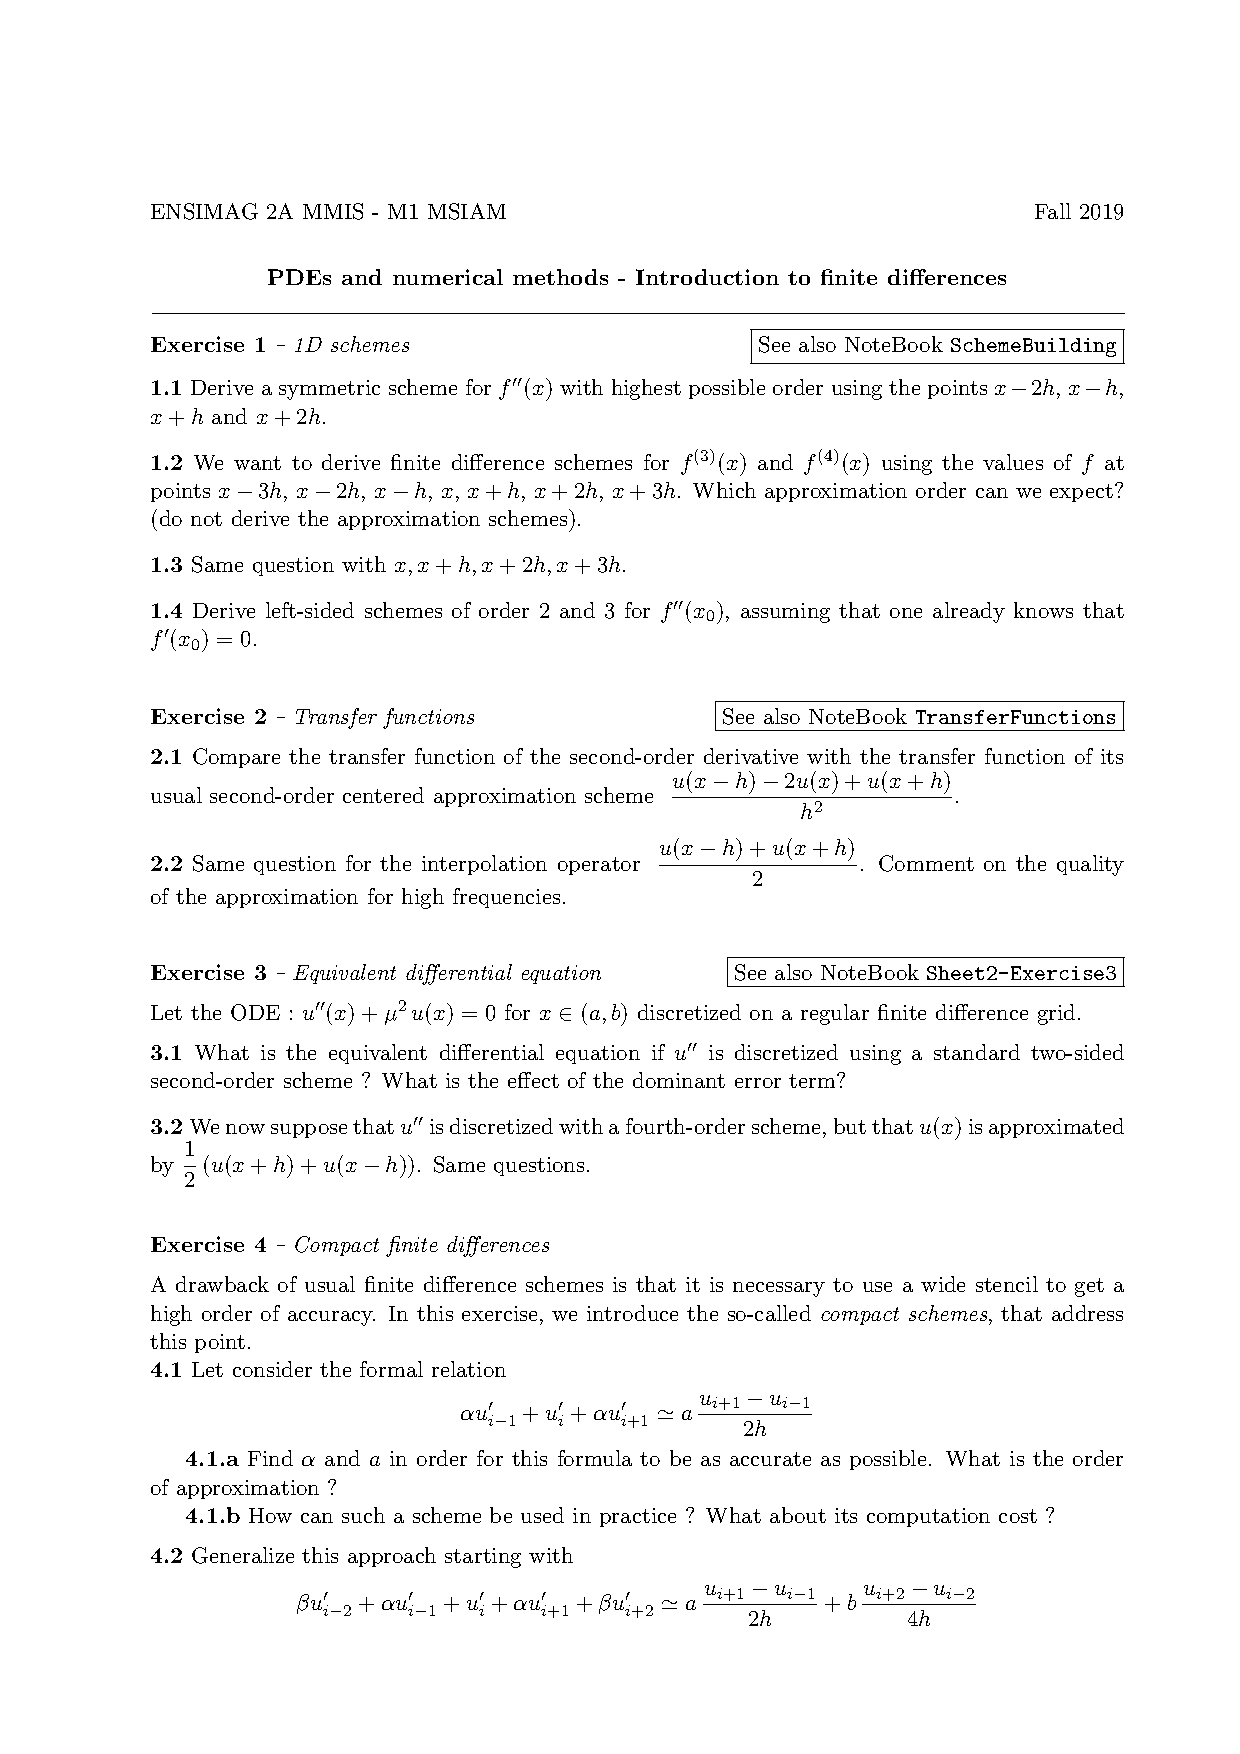
\includepdf[pages=-]{sources/td2.pdf}
\section{Exercise sheet 2}
\label{sec:Exercise sheet 2}
\subsection{1D schemes}
\label{subsec:1D schemes}
\subsubsection{1.1}
Derive a symmetric scheme for $ f''(x) $ with the highest possible order using the points,
$ x-2h, x-h, x+h, x+2h $. 
We have $ p = 2, q = 4 $, using the Taylor formula we have 
\begin{align*}
        f(x-2h) &= f(x) - 2hf'(x) + \frac{ 4h^2f''(x)  }{ 2 } - \frac{ 8h^3f'''(x)  }{ 6 } +
        \frac{ 16h^4f^{4}(x)  }{ 24 } \\ 
        f(x-h) &= f(x) + hf'(x) + \frac{ h^2f''(x)  }{ 2 } + \frac{ h^3f'''(x)  }{ 6 } +
        \frac{ h^4f^{4}(x)  }{ 24 } \\ 
        f(x+h) &= f(x) - hf'(x) + \frac{ h^2f''(x)  }{ 2 } - \frac{ h^3f'''(x)  }{ 6 } +
        \frac{ h^4f^{4}(x)  }{ 24 } \\ 
        f(x+2h) &= f(x) + 2hf'(x) + \frac{ 4h^2f''(x)  }{ 2 } + \frac{ 8h^3f'''(x)  }{ 6 } +
        \frac{ 16h^4f^{4}(x)  }{ 24 }  
\end{align*}

which gives us the Vandermonde matrix 
\[
\begin{pmatrix*}[r]
    -2& -1& 1& 2&\\
    4& 4& 1& 4&\\
    -8& -1& 1& 8&\\
    16& 1& 1& 16&
\end{pmatrix*}
\begin{pmatrix*}[r]
    \beta_1 \\
     \beta_2\\
     \beta_3\\
     \beta_4
\end{pmatrix*}
= \begin{pmatrix*}[r]
     0 \\
     2 \\
     0 \\
     0
\end{pmatrix*}
\]
We solve it directly using the augmented matrix : 
\begin{align*}
\begin{pmatrix*}[r]
    -2& -1& 1& 2&\\[0.5em]
    4& 4& 1& 4&\\[0.5em]
    -8& -1& 1& 8&\\[0.5em]
    16& 1& 1& 16&
\end{pmatrix*}
     &\implies  
     \begin{pmatrix}[cccc|c]
         -1& - \frac{ 1 }{ 2 }& \frac{ 1 }{ 2 } & 1& 0\\[0.5em]
         1&  \frac{ 1 }{ 4 }& \frac{ 1 }{ 4 } & 1& \frac{ 1 }{ 2 } \\[0.5em]
         -1& - \frac{ 1 }{ 8 }& \frac{ 1 }{ 8 } & 1& 0\\[0.5em]
         -1&  \frac{ 1 }{ 16 }& \frac{ 1 }{ 16 } & 1& 0
\end{pmatrix} \\ 
         R_3 - R_1 \text{ and } R_4 - R_2  &\implies \\ 
         \begin{pmatrix}[cccc|c]
         -1& - \frac{ 1 }{ 2 }& \frac{ 1 }{ 2 } & 1& 0\\[0.5em]
         1&  \frac{ 1 }{ 4 }& \frac{ 1 }{ 4 } & 1& \frac{ 1 }{ 2 } \\[0.5em]
         0&  \frac{ 3 }{ 8 }& -\frac{ 3 }{ 8 } & 0& 0\\[0.5em]
         0&  -\frac{ 3 }{ 16 }& -\frac{ 3 }{ 16 } & 0& -\frac{ 1 }{ 2 } 
     \end{pmatrix} \quad &\implies 
\begin{pmatrix}[cccc|c]
         -1& - \frac{ 1 }{ 2 }& \frac{ 1 }{ 2 } & 1& 0\\[0.5em]
         1&  \frac{ 1 }{ 4 }& \frac{ 1 }{ 4 } & 1& \frac{ 1 }{ 2 } \\[0.5em]
         0&  1& - 1& 0& 0 \\[0.5em]
         0&  1&  1& 0& \frac{ 8 }{ 3 } 
     \end{pmatrix} 
\end{align*}
By $ R_3, R_4 $ we know that $ \beta_2 = \beta_3 $ and $ 2\beta_2 = \frac{ 4 }{ 3 } =
\beta_3 $. By $ R_1 $ we have $ \beta_1 = \beta_4 $ and by $ R_2,\  2\beta_1 + \frac{ 4 }{12 } =
\frac{ 1 }{ 2 } \implies \beta_1 = -\frac{ 1 }{ 12 } = \beta_4$ 
Thus, 
\[
\beta = \begin{pmatrix*}[r]
    - \frac{ 1 }{ 12 }  \\[0.5em]
    \frac{ 4 }{ 3 } \\[0.5em]
    \frac{ 4 }{ 3 } \\[0.5em]
    -\frac{ 1 }{ 12 } 
\end{pmatrix*}

\]

applying these coefficients to the equations we have 
\begin{align*}
     - \frac{ 1 }{ 12 } f(x-2h) &= -\frac{ 1 }{ 12 }  f(x) + \frac{ 1 }{ 6 }hf'(x) - 
     \frac{ h^2f''(x)  }{ 6 } + \frac{ h^3f'''(x)  }{ 9 } -
        \frac{ h^4f^{4}(x)  }{ 18 } \\ 
     \frac{ 4 }{ 3 }    f(x-h) &= \frac{ 4 }{ 3 } f(x) - \frac{ 4 }{ 3 } hf'(x) 
     + \frac{ 2 }{ 3 } h^2f''(x)  +  \frac{ 2h^3f'''(x)  }{ 9 } + \frac{ h^4f^{4}(x)  }{
     18 } \\ 
     \frac{ 4 }{ 3 }    f(x+h) &= \frac{ 4 }{ 3 } f(x) + \frac{ 4 }{ 3 } hf'(x) 
     + \frac{ 2 }{ 3 } h^2f''(x)  -  \frac{ 2h^3f'''(x)  }{ 9 } + \frac{ h^4f^{4}(x)  }{
     18 } \\ 
     - \frac{ 1 }{ 12 } f(x-2h) &= -\frac{ 1 }{ 12 }  f(x) - \frac{ 1 }{ 6 }hf'(x) - 
     \frac{ h^2f''(x)  }{ 6 } - \frac{ h^3f'''(x)  }{ 9 } -
        \frac{ h^4f^{4}(x)  }{ 18 } \\ 
\end{align*}
This gives 
\[
    \frac{ 30 }{ 12 } f(x) + h^2 f''(x) + \mathcal{ O } \left( h^5\right)   
\]

which results in the scheme  
\[
    u''(x) = \frac{ -f(x-2h) + 16f(x-h) + 30f(x) + 16f(x+h) - f(x+2h)     }{ 12h^2 } 
\]

\subsubsection{1.2}
Since we have symmetric schemes we can use the formula to find the approximation order. 
\[
p + 2 - q = \text{approx Order} 
\]
where $ p =  $ the points of the stencil (not including $ f(x)  $) and q is the order we
want to find. Thus, for $ f^{(3)}(x)  $ we have 
\[
6 + 2 - 3 = 5
\]
and for $ f^{(4)}  $ we have 
\[
6 + 2 - - 4 = 4
\]

\subsubsection{1.3}
We no longer have a symmetric scheme. Therefore, we use the formula 
\[
p + 1 - q = \text{approx Order} 
\]
Our stencil is $ x, x+h, x+2h, x+3h $. Thus, for $ f _{  }^{ (3) } (x) $ we have 
\[
3 + 1 - 3 = 1
\]
and for $ f _{  }^{ (4) } (x) $ we have 
\[
3 + 1 - 4 = 0
\] which does not converge not matter what h is chosen. 

\subsection{Transfer Functions }
\label{subsec:Transfer Functions }
\subsubsection{2.1}
We first find the exact transfer function of $ u''(x) $, given by 
\[
    S \left( u_{\omega} \right) \left( x\right) = \left( e _{  }^{ i\omega x } \right) ''
    = -\omega^2 e _{  }^{ i\omega x } = -\omega^2 u _{ \omega }^{  } 
\] 
so we can say that the transfer function is 
\[
T\left( \omega\right) = -\omega^2
\]

The scheme to analyze is 
\[
\frac{ u(x-h) - 2u(x) + u(x_h)  }{ h^2 } 
\]
and 
\begin{align*}
   &e^{ i\omega\left( x-1\right) } - 2 e^{ i\omega x} + e^{ i\omega\left( x+1\right) } \\ 
    & e^{ i\omega x} \left( e^{ -i\omega } - 2 + e^{ i\omega }  \right)  \\ 
    & u _{ \omega }^{  } \left( 2\cos(\omega) - 2\right)   \\ 
    & -4\sin^2\left( \frac{ \omega }{ 2 } \right)u_{\omega}  \\ 
\end{align*}
This gives 
\[
T_1\left( \omega \right) = 2\left( 1 - \frac{ \omega^2 }{ 2 } + \frac{ \omega^4 }{ 4  } +
\mathcal{ O  } \left( \omega^5\right) \right) - 2
\]
\[
= -\omega^2 + \frac{ \omega }{ 12 } + \mathcal{ O  } \left( \omega ^5\right) 
\]

This scheme is dissipative due to the fact that the amplitude has been altered.


\subsubsection{2.2}
Consider 
\[
    \frac{ u(x-h) + u(x+h)  }{ 2 } 
\]

which is a scheme for finding $ f' $. Thus, the exact spectral analysis gives, 
\[
    S(u_\omega)(x) = \left( e^{ i\omega x} \right) ' = i\omega e^{ i\omega x} = i\omega
    u_\omega
\]
with transfer function : 
\[
    T(\omega) = i\omega
\]
\begin{align*}
    &\frac{ e^{ i\omega\left( x-1\right) } + e^{ i\omega\left( x+1\right) }  }{ 2 } \\
     & \frac{ 1 }{ 2 } e^{ i\omega x} \left( e^{ -i\omega} + e^{ i\omega} \right)  \\ 
     & e^{ i\omega x} \frac{ 1 }{ 2 } \left( e^{ i\omega} + e^{ -i\omega} \right)  \\
     & e^{ i\omega x } \cos(\omega) \\ 
\end{align*}
which gives 
\[
    T_1(\omega) = \cos \omega 
\]

Since $\omega \in [0,\pi]$ we can see that, the greater $ \omega $, the smaller h must be. 

\subsection{Excercise 3 : Equivalent differential equation}
\label{subsec:Excercise 3 : Equivalent differential equation}
Consider 
\begin{equation}
    u''(x) + \mu^2 u(x) = 0 \quad \text{ for } x \in [a,b] 
    \label{eq:equiv_diff_eq}
\end{equation}
discretized on a regular finite difference grid. 
\subsubsection{3.1}
What is the equivalent ODE? 
$ \\ $If we have a standard two-sided second-order scheme then 
\[
    u''(x) \approx \frac{ u(x+h) -2u(x) + u(x-h)  }{ 2 } + \frac{ h^2 }{ 12 } u _{  }^{
    (4) } (x) + \mathcal{ O  } (h^4) 
\]
substituting into \ref{eq:equiv_diff_eq} we get 
\begin{equation}
    \frac{ u(x+h) -2u + u(x-h)  }{ h^2 } + \mu^2 u = 0
    \label{eq:3.1_Sh}
    \tag{S_h}  
\end{equation}
and  
\[
    \frac{ h^2 }{ 12 } u _{  }^{ (4) } + u'' + \mu^2 u = 0
\]
This ODE is close to $ \left( S_h\right)  $ up to a 4th order, while the original equation
is up to only a 2nd order. Thus, inspection of analytic solutions will give us some
insight to the numerical solution of $ \left( S_h\right)  $.
$ \\ $Solution to the ODE
\[
\frac{ h^2  }{ 12 } X^4 + X^2 + \mu^2 = 0
\]

Let $ Y = X^2 $, 
\[
\frac{ h^2 }{ 12 } Y^2 + Y + \mu^2 = 0 
\]
Using quadratic formula, 
\[
    \frac{ 1 \pm \sqrt{1 - \frac{ h^2\mu^2 }{ 3 }   }}{ \frac{ h^2 }{ 6 }  } 
\]
which gives 
\[
    R_1 = \frac{ 6 }{ h^2 } \left( 1 + \sqrt{1 - \frac{ h^2\mu^2 }{ 3 }   } \right) 
\qquad 
    R_2 = \frac{ 6 }{ h^2 } \left( 1 - \sqrt{1 - \frac{ h^2\mu^2 }{ 3 }   } \right) 
\]
Therefore, 
\[
    X = \pm ir_j \qquad r_j = \sqrt{-R_j} \qquad j = 1,2
\]


\subsection{Compact Finite Differences}
\label{subsec:Compact Finite Differences}
\begin{equation}
    \alpha u' _{i-1} + u'_i + \alpha u'_{i+1} \approx a \frac{ u_{i+1} - u_{i-1} }{ 2h } 
    \label{eq:compact_FD}
\end{equation}
\subsubsection{1.a}
Find $ \alpha  $ and a in order for this formula to be as accurate as possible. What is
the order of approximation? 

We first expand the right hand side of \ref{eq:compact_FD}  
\[
    a \frac{ u_{i+1} - u_{i-1} }{ 2h } = u' + \frac{ h^2  }{ 6 } u^{(3)} + \mathcal{ O  }
    \left( h^5 \right) 
\]
Similarly, we have for the left hand side
\begin{align*}
    \alpha u'_{i-1}  &= u'(x) -hu''(x) + \frac{ h^2 }{ 2 }  u _{  }^{ (3) } (x) - \frac{
    h^3 }{ 6 } u^{(4)} (x) + \mathcal{ O  } \left( h^4\right) \\
        \alpha u'_{i+1}  &= u'(x) + hu''(x) + \frac{ h^2 }{ 2 }  u _{  }^{ (3) } (x) + \frac{
    h^3 }{ 6 } u^{(4)} (x) + \mathcal{ O  } \left( h^4\right) 
\end{align*} 
We cancel the 2nd and 4th order terms.
Finally, 

\begin{align*}
    \alpha \left( 2u'(x) + h^2u^{(3)}(x) \right) + u'_i &\approx au' + a\frac{ h^2  }{ 6 } u^{(3)}\\
    u'(x)\left( 2\alpha + 1\right) + \alpha u^{(3)}(x) &\approx   au' + a\frac{ h^2  }{ 6 } u^{(3)}\\ 
\end{align*}
With some simple algebra we have 
\begin{align*}
    2\alpha + 1 = a &\qquad \alpha = \frac{ a }{ 6 }  \\
    a = \frac{ 3 }{ 2 }  &\qquad  \alpha = \frac{ 1 }{ 4 } \\
\end{align*}
Plugging into the original equation gives 
\[
    \frac{ 1 }{ 4 }  u' _{i-1} + u'_i + \frac{ 1 }{ 4 } u'_{i+1} \approx \frac{ 3 }{ 2 }
    \frac{ u_{i+1} - u_{i-1} }{ 4h } 
\]

The left hand side of \ref{eq:compact_FD} is of of 4th order accuracy and the right is of 5th order
accuracy, this results in a final solution having 4th order accuracy. 



\subsection{Shooting method}
\label{subsec:Shooting method}


\subsection{2D Laplacian}
\label{subsec:2D Laplacian}
\subsubsection{a)}
\begin{aligned }
    \[f(x+h,y) &= f(x,y) + h \partial_xf(x+h,y) + \frac{ h^2 \partial_{x^2}f(x+h,y) }{ 2 } + \mathcal{ O  } (h^2)
    \\ \]
    \[f(x-h,y) &= f(x,y) - h \partial_xf'(x+h,y) + \frac{ h^2 \partial_{x^2}f(x+h,y) }{ 2 } + \mathcal{ O  } (h^2)
\\ \]
\[f(x,y+k) &= f(x,y) + k \partial_yf(x,y+k) + \frac{ k^2 \partial_{y^2} f(x,y+k) }{ 2 } + \mathcal{ O  } (h^2)
\\ \]
\[ f(x,y-k) &= f(x,y) - k \partial_yf(x,y-k) + \frac{ k^2 \partial_{y^2}f(x,y-k) }{ 2 } + \mathcal{ O  } (h^2)
\\ \]
\end{aligned}
which gives us 
\[
    \frac{ f(x+h, y) - 2f(x,y) + f(x-h, y)  }{ h^2 } + \mathcal{ O  } (h^2) +  \frac{
   f(x, y+k) - 2f(x,y) + f(x, y-k)  }{ k^2 } + \mathcal{ O  } (k^2)
\]
\subsubsection{b)}
We simplify the above scheme to 
\[
    \frac{ f(x+h, y) + f(x-h, y) -4f(x,y) + f(x,y+h) + f(x,y-h) }{ h^2 } + \mathcal{ O  }
    (h^2)
\]
We now wish to derive another scheme using the other five gridpoints. 
\newpage
\begin{aligned }
    \[f(x+h,y+k) &= f(x,y) + h \partial_xf(x+h,y+k) + k \partial_yf(x+h,y+k) + 
    \frac{ h^2 \partial_{x^2}f(x+h,y+k) }{ 2 } \\ \] 
    \[ &+ \frac{ hk \partial_{xy}f(x+h,y+k) }{ 2 } +
        \frac{ k^2 \partial_{y^2}f(x+h,y+k) }{ 2 } 
        + \mathcal{ O  } (h^2,k^2)
    \\ \]
    \[f(x+h,y-k) &= f(x,y) + h \partial_xf(x+h,y+k) - k \partial_yf(x+h,y-k) + 
    \frac{ h^2 \partial_{x^2}f(x+h,y-k) }{ 2 } \\ \] 
    \[ &- \frac{ hk \partial_{xy}f(x+h,y-k) }{ 2 } +
        \frac{ k^2 \partial_{y^2}f(x+h,y-k) }{ 2 } 
        + \mathcal{ O  } (h^2,k^2)
    \\ \]
    \[f(x-h,y+k) &= f(x,y) - h \partial_xf(x-h,y+k) + k \partial_yf(x-h,y+k) + 
    \frac{ h^2 \partial_{x^2}f(x-h,y+k) }{ 2 } \\ \] 
    \[ &- \frac{ hk \partial_{xy}f(x-h,y+k) }{ 2 } +
        \frac{ k^2 \partial_{y^2}f(x-h,y+k) }{ 2 } 
        + \mathcal{ O  } (h^2,k^2)
    \\ \]
    \[f(x-h,y-k) &= f(x,y) - h \partial_xf(x-h,y-k) - k \partial_yf(x-h,y-k) + 
    \frac{ h^2 \partial_{x^2}f(x-h,y-k) }{ 2 } \\ \] 
    \[ &+ \frac{ hk \partial_{xy}f(x-h,y-k) }{ 2 } +
        \frac{ k^2 \partial_{y^2}f(x-h,y-k) }{ 2 } 
        + \mathcal{ O  } (h^2,k^2)
    \\ \]
\end{aligned}
Adding these all together we have 
\[
    4f(x,y) + 2h^2 \partial _{x^2} f + 2k^2 \partial _{y^2} f + \mathcal{ O  } \left( h^2,
    k^2 \right) 
\]
Thus, 
\[
    \frac{ f(x+h, y+k) + f(x+h, y-k) - 4f(x,y) + f(x-h, y+k) + f(x+h, y-k)  }{ h^2 } +
    \mathcal{ O }\left( h^2, k^2\right)  
\]

\subsubsection{c)}
In the 1st scheme, when we try to expand we have $ \partial _{ x }^{ (4) } f $ and $
\partial _{ y }^{ (4) } f $ in the error term. In the second scheme we get error terms
involving $ \partial _{ xxyy }^{ (4) } f $ which cannot be canceled. Thus we cannot get a
higher order scheme using a combination of these two.

\subsection{Exercise 7 : 2D Taylor Formula}
\label{subsec:Exercise 7 : 2D Taylor Formula}

